%\renewcommand{\footrulewidth}{0.5pt}% default is 0pt
%\lfoot{\textcolor{darkgray}{Curriculum Vitae -- Prof.\ Dr.\ Han van der Aa}}
%\rfoot{\textcolor{darkgray}{\monthyeardate\today}}
%
%\makesavenoteenv{tabular}
%
	\newpage
\phantomsection
\addcontentsline{toc}{chapter}{Curriculum Vitae}
\lfoot{\textcolor{darkgray}{Curriculum Vitae -- Han van der Aa}}

\begin{paracol}{1} % Begin the multi-column environment



\parbox[top][0.12\textheight][c]{\linewidth}{ % Parbox to hold the author name and CV text; fixed height to match the coloured box to the right, centred vertically and full line width
	\vspace{-0.04\textheight} % Reduce whitespace above the parbox to separate it from the main content
	\centering % Centre text
	{\sffamily\Huge Prof.\ Dr.\ Han van der Aa}\\\medskip % Your name
	{\huge\color{headings} Curriculum Vitae }
}
%\switchcolumn
\end{paracol}
\vspace{0.3em}
\begin{paracol}{2}
	\hspace{2em}
\parbox[top][0.12\textheight][c]{1.00\linewidth}{ % Parbox to hold the colour box; fixed height to match the name/CV text to the left, centred vertically and full line width
	\vspace{-0.04\textheight} % Reduce whitespace above the parbox to separate it from the main content
	\colorbox{white}{ % Create the coloured box
		\begin{supertabular}{ll} % Start a table with two columns, the table will ensure everything is aligned
			\raisebox{-1pt}{Full name} & Johannes Hendrikus van der Aa \\ %
			\raisebox{-1pt}{Date of Birth} & 9 October 1988 \\ %
			\raisebox{-1pt}{Place of Birth} & Sint-Oedenrode, the Netherlands \\ %
			\raisebox{-1pt}{Address} & Hafenstrasse 31, 68159, Mannheim, Germany \\ % Address
			\raisebox{-1pt}{Phone:} & +49 (1) 763 460 1322 \\ % Phone number
			\raisebox{-1pt}{E-mail} & \href{mailto:han@informatik.uni-mannheim.de}{han@informatik.uni-mannheim.de} \\ % Email address
			\raisebox{0pt}{Homepage} & \href{https://www.hanvanderaa.com}{www.hanvanderaa.com} \\ % 
		\end{supertabular}
	}
}
\switchcolumn
%\begin{figure}
\vspace{-1.5em}
\hspace{12em}
	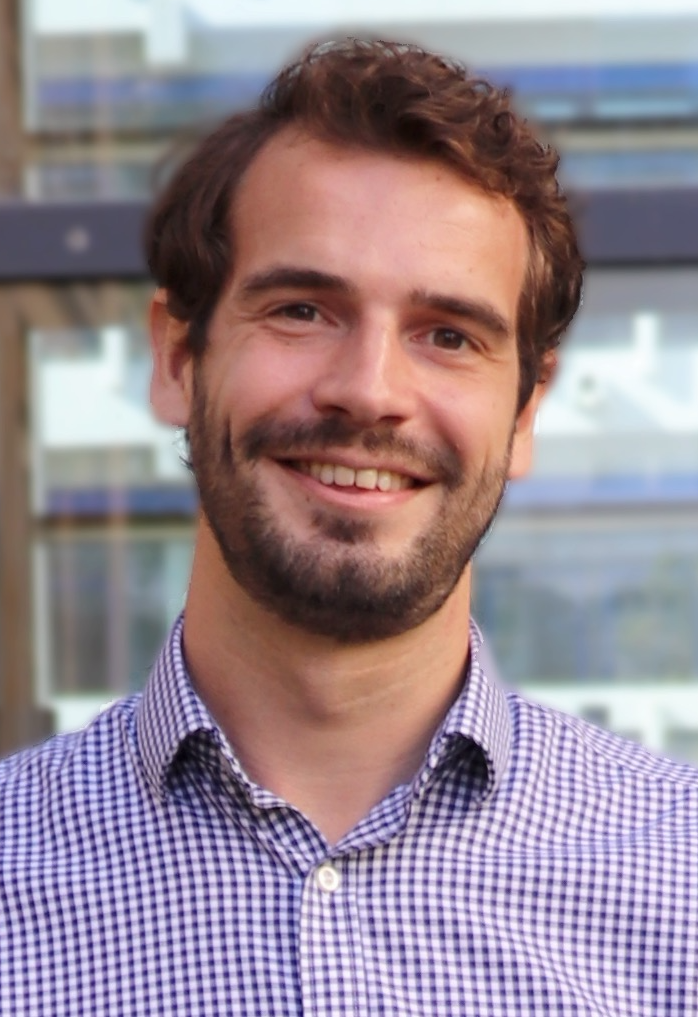
\includegraphics[height=3.3cm]{figures/headshot.png}
%\end{figure}

\end{paracol}

\medskip
\vspace{0.3em}
\section{Work Experience}
\begin{tabular}{p{12.5cm}l}
		\normalsize \textbf{Junior Professor in Artificial Intelligence Methods} & 		04/2020 -- current\\
		Head of the research group on Process Analytics \\
			Funded by the \textit{Künstliche Intelligenz Baden-Württemberg} (KI-BW) initiative \\ 
 School of Business Informatics and Mathematics \\
 	University of Mannheim, Germany \\
	\noalign{\smallskip\smallskip}
	
	\normalsize \textbf{Alexander von Humboldt Fellow (post-doctoral researcher)} & 			05/2018  --  03/2020 \\
	Databases \& Information Systems Group, Department of Computer Science\\
		Humboldt-Universit\"at zu Berlin, Germany \\
	\noalign{\smallskip\smallskip}
	
	\normalsize \textbf{Post-doctoral Researcher} & 		01/2018  --  04/2018 \\
	Business Informatics Group, Department of Computer Sciences \\
		Vrije Universiteit Amsterdam, the Netherlands \\
	\noalign{\smallskip\smallskip}
	
	
	\normalsize \textbf{Ph.D. Candidate} & 05/2014  --  01/2018 \\
	Business Informatics Group, Department of Computer Sciences \\
	Vrije Universiteit Amsterdam, the Netherlands \\
	\noalign{\smallskip\smallskip}
	
	\normalsize \textbf{Junior Researcher} & 09/2013  --  02/2014 \\
	SAP AG, Germany \\
%	Joint research in collaboration with the Eindhoven University of Technology\\
	
\end{tabular}


\medskip
\vspace{0.3em}
\section{Education}
\begin{tabular}{p{12.5cm}l}
 \normalsize \textbf{Ph.D. in Computer Science } & 	05/2014  --  01/2018 \\
	 Vrije Universiteit Amsterdam, the Netherlands \\
	 Thesis: \textit{Comparing and Aligning Process Representations} \\
%	 Supervisors: Prof.\ Dr.\ Hajo A. Reijers and Dr.\ Henrik Leopold \\
	 Honors: \textit{cum laude} (top 5\% in the Netherlands) \\
	\noalign{\smallskip\smallskip}
	
	 \normalsize \textbf{M.Sc. in Business Information Systems } & 09/2010  --  04/2013\\
	 Eindhoven University of Technology, the Netherlands \\
	 Thesis: \textit{Composing Workflow Activities} \\
	Honors: \textit{cum laude} (top 5\% of the university) \\
	\noalign{\smallskip\smallskip}

	
	 \normalsize \textbf{B.Sc. in Industrial Engineering } & 09/2007  --  07/2010 \\
	 Eindhoven University of Technology, the Netherlands \\
	 Honors: \textit{cum laude} (top 5\% of the university)
		
\end{tabular}

\section{Research Visits}
\begin{tabular}{p{12.5cm} p{3cm}  }
	\textbf{Universit\'e Paris Dauphine, France -- Visiting professor} & 10/2021 -- current  \\
	LAMSADE Laboratory \\
	\noalign{\smallskip\smallskip}
	
	\textbf{Technion - Israel Institute of Technology, Israel -- Visiting researcher} & 11/2017 -- 12/2017 \\
	Faculty of Industrial Engineering \& Management \\
	%	 Work on instance-based process matching with Prof.\ Dr.\ Avigdor Gal \\
	\noalign{\smallskip\smallskip}
	
	\textbf{Vienna Univ. of Economics and Business, Austria -- Visiting researcher} & 06/2013 -- 08/2013\\
	Department of Information Systems and Operations \\
	%	 Work on anomaly detection in flight trajectories with Prof.\ Dr.\ Jan Mendling \\
\end{tabular}


\section{Awards}
\begin{tabular}{lll  }
	\normalsize \textbf{Best student paper} &
	Int. conf. on Conceptual Modeling (ER) & 2020 \\
	
	\normalsize \textbf{Runner-up best paper} &
	Int. conf.  on Business Process Management (BPM) & 2019 \\
	\normalsize \textbf{Runner-up best thesis} &
	Int. conf. on Business Process Management (BPM) & 2018\\
	\normalsize \textbf{Runner-up best paper} & 
	Int. conf.  on Advanced Information Systems Engineering (CAiSE) & 2017\\
	
\end{tabular}

\medskip 

\section{Acquisition of Third-Party Funds}
\begin{tabular}{p{1.3cm}p{10.8cm}l}
	\multicolumn{2}{l}{\normalsize \textbf{Alexander von Humboldt Fellowship}} & 05/2018 -- 04/2020\\
	Agency: &Alexander von Humboldt Foundation \\
	Call: & Research Fellowships for post-doctoral researchers \\
	Proposal: & Temporal Uncertainty in Conformance Checking of Business Processes \\
	Role: & Principal Investigator  \\
	Amount: & \small\textbf{85,500 EUR} \\
	
\end{tabular}



\medskip
\section{Invited Talks }

	\textbf{Research Talks}
	\smallskip
	
\begin{tabular}{p{13.5cm}l}

	
\textbf{Challenges and Opportunities of Natural Language Processing in BPM} & 12/2019 \\	
{University of Seville, Spain}  \\
	\noalign{\smallskip\smallskip}

\textbf{Complex Event Processing for Event-Based Process Querying} (keynote) & 09/2019 \\
{International Workshop on Process Querying} \\
	\noalign{\smallskip\smallskip}

\textbf{Process Mining for Automated Compliance Checking} & 11/2017\\	
	{ING Bank, Amsterdam, the Netherlands}  \\

	\noalign{\smallskip\smallskip}
	
\textbf{Comparing Textual Process Descriptions to Process Models} & 01/2017\\
	{Technical University of Barcelona, Spain} \\

	\noalign{\smallskip\smallskip}

	\textbf{An introduction to Process Model Matching} (guest lecture) & 11/2016 \\	
	{Technion -- Israel Institute of Technology, Haifa, Israel}  \\

	\noalign{\smallskip\smallskip}
\textbf{Detecting Inconsistencies between Process Models and Textual Descriptions} & 11/2014 \\
	{Vienna University of Economics and Business, Austria} \\

	
\end{tabular}

\medskip
\textbf{Tutorials} 
\smallskip 
 
\begin{tabular}{p{13.5cm}l}
	
	
	\textbf{RuM: Declarative Process Mining, Distilled} & 09/2021  \\
%	With Anti Alman, Claudio di Ciccio, Marco Montali, and Fabrizio M. Maggi \\
	Int. Conf. on Business Process Management \\
	\noalign{\smallskip\smallskip}
	
		\textbf{Process Mining: Leveraging Event Data to Understand and Improve Organizations} & 12/2019 \\
%	With Henrik Leopold \\
	IEEE Int. Conf. on Big Data \\
	\noalign{\smallskip\smallskip}

\end{tabular}


\medskip
\section[Scientific Service]{Scientific Service (Selection)}


\textbf{Track Chair} 
\smallskip 

\begin{tabular}{p{13.5cm}l}
%	\textbf{Track Chair} \\
	HICSS Mini-Track on Business Process Technology & \hphantom{2020 - }2022 \\
		\noalign{\smallskip\smallskip}
\end{tabular}

\textbf{Program Committees}

\begin{tabular}{p{13.5cm}l}
	
		Int. conf. on Process Mining (ICPM) & \hphantom{2020 - }2021 \\
			Int. conf on Distributed and Event-Based Systems (DEBS) & \hphantom{2020 - }2021  \\
	Int. conf. on Business Process Management (BPM) & 2020 - 2021 \\
Int. working conf. on Business Process Modeling, Development, and Support (BPMDS) & 2019 -- 2021 \\
		International Joint Conference on Neural Networks (IJCNN) & \hphantom{2020 - }2020 \\
		
	\noalign{\smallskip\smallskip}
Workshop on Process Querying & 2019 -- 2021\\

		Workshop on Artificial Intelligence for Business Process Management  & 2018 -- 2021\\
Workshop on Declarative/Decision/Hybrid Mining and Modelling for Business Processes & 2018 -- 2021\\
Workshop on Blockchains for Inter-Organizational Collaboration & \hphantom{2020 - }2018\\
Workshop on Cognitive Business Process Management & \hphantom{2020 - }2017 \\
\end{tabular}

\newpage 
\textbf{Reviewer for Journals}
\smallskip 

\begin{tabular}{p{1.7cm}p{10.5cm}l}
	 	BISE & Business \& Information Systems Engineering \\
	 	COMIND & Computers in Industry \\
	 	COMP & Computing \\ 
 	 	DSS &  	Decision Support Systems \\
 	 	ESWA & Expert Systems with Applications \\ 
	 	IS & Information Systems \\
	 	JODS & Journal on Data Semantics \\
	 	SoSym & Software and Systems Modeling \\
	 	TKDE & IEEE Transactions on Knowledge and Data Engineering \\
\end{tabular}

\smallskip 
\textbf{Reviewer for Conferences}
\smallskip	

\begin{tabular}{p{1.7cm}p{11.3cm}l}
	
HICSS &	Hawaii International Conference on System Sciences &  \hphantom{2018 -- }2021 \\
	ECIS &	European Conference on Information Systems&  2018 -- 2021 \\
	AMCIS & 	Americas Conference on Information Systems &  \hphantom{2018 -- }2017 \\
		BPMDS & Business Process Modeling, Development, and Support &  2015 --  2017 \\
%		SAC &  ACM Symposium on Applied Computing & 2017 \\
		WI & International Conference on Wirtschaftsinformatik & \hphantom{2018 -- }2017 \\
		ICSOC & International Conference on Service Oriented Computing &  2015 -- 2016 \\
%		BPM & International Conference on Business Process Management &  2016 \\
\end{tabular}

\smallskip
\textbf{Reviewer for Funding Agencies}
\smallskip

\begin{tabular}{p{1.7cm}p{11.3cm}l}
SNF & Swiss National Science Foundation \\
\end{tabular}


